\documentclass[10pt]{article}
\usepackage[ngerman]{babel}
\usepackage[utf8]{inputenc}
\usepackage[T1]{fontenc}
\usepackage{amsmath}
\usepackage{amsfonts}
\usepackage{amssymb}
\usepackage[version=4]{mhchem}
\usepackage{stmaryrd}
\usepackage{graphicx}
\usepackage[export]{adjustbox}
\graphicspath{ {./images/} }

\title{Hauptprüfung Abiturprüfung 2021 - Leistungsfach }

\author{Alexander Schwarz\\
www.mathe-aufgaben.com}
\date{}


\begin{document}
\maketitle
 Baden-WürttembergAugust 2021

\section*{Aufgabe B1}
Gegeben ist eine gerade Pyramide mit quadratischer Grundfläche.\\
Die Eckpunkte der Grundfläche sind $\mathrm{A}(-3|-3| 0), \mathrm{B}(3|-3| 0), \mathrm{C}(3|3| 0)$ und D , die Spitze ist $\mathrm{S}(0|0| 6)$.\\
Die Ebene E enthält die Punkte A, B und S.\\
a) Stellen Sie die Pyramide in einem geeigneten Koordinatensystem dar. (1 VP)\\
Bestimmen Sie eine Koordinatengleichung der Ebene E .\\
$(2 \mathrm{VP})$

Berechnen Sie den Oberflächeninhalt der Pyramide.\\
(Teilergebnis: E: $2 x_{2}-x_{3}=-6$ )\\
b) Innerhalb der Pyramide gibt es einen Punkt, dessen Abstand von der Grundfläche der Pyramide $\sqrt{5}$-mal so groß ist wie sein Abstand zu den Seitenflächen. Berechnen Sie die Koordinaten dieses Punktes.\\
c) Betrachtet wird für jedes a $>0$ die gerade Pyramide mit folgenden Eigenschaften:

\begin{itemize}
  \item $A(-a|-a| 0), B(a|-a| 0), C(a|a| 0)$ und $D$ sind die Eckpunkte der quadratischen Grundfläche.
  \item Die $x_{3}$-Koordinate der Spitze $S$ ist positiv.
  \item Die Höhe der Pyramide stimmt mit der Kantenlänge der Grundfläche überein.\\
$M_{1}$ ist die Kantenmitte von $A B, M_{2}$ die Kantenmitte von DS.\\
Zeigen Sie: Die Strecke $\mathrm{M}_{1} \mathrm{M}_{2}$ ist orthogonal zur Kante DS.
\end{itemize}

\section*{Lösungen}
\section*{Aufgabe B1}
a) Stellen Sie die Pyramide in einem geeigneten Koordinatensystem dar.\\
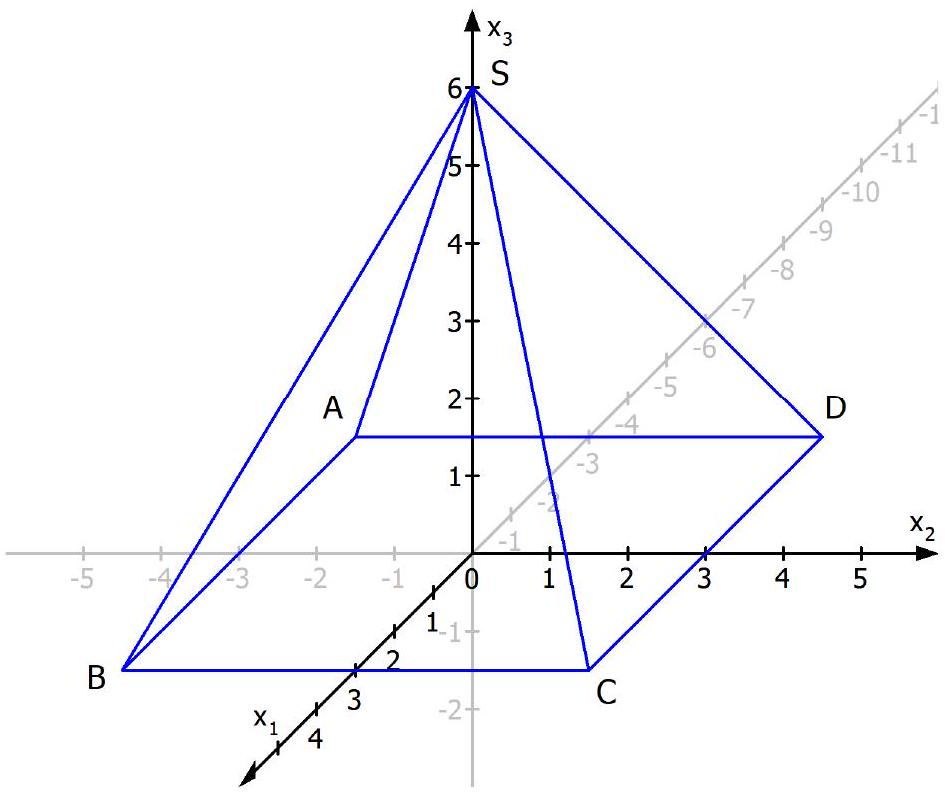
\includegraphics[max width=\textwidth, center]{2025_04_24_14f10423eb24445411eeg-3}

Bestimmen Sie eine Koordinatengleichung der Ebene E.\\
Parameterform der Ebene $E: \vec{x}=\left(\begin{array}{c}-3 \\ -3 \\ 0\end{array}\right)+r \cdot\left(\begin{array}{l}6 \\ 0 \\ 0\end{array}\right)+s \cdot\left(\begin{array}{l}3 \\ 3 \\ 6\end{array}\right)$\\
Normalenvektor von $E: \vec{n}=\left(\begin{array}{l}6 \\ 0 \\ 0\end{array}\right) \times\left(\begin{array}{l}3 \\ 3 \\ 6\end{array}\right)=\left(\begin{array}{c}0 \\ -36 \\ 18\end{array}\right)$ bzw- $\overrightarrow{\mathrm{n}}^{*}=\left(\begin{array}{c}0 \\ 2 \\ -1\end{array}\right)$\\
Ansatz für Koordinatengleichung: $\mathrm{E}: 2 \mathrm{x}_{2}-\mathrm{x}_{3}=\mathrm{d}$\\
Einsetzen des Punktes A(-3|-3|0): $-6=\mathrm{d}$\\
Koordinatengleichung: $E: 2 x_{2}-x_{3}=-6$

Berechnen Sie den Oberflächeninhalt der Pyramide.\\
Die Grundfläche der Pyramide hat einen Inhalt von $G=6 \cdot 6=36$ FE

Flächeninhalt des Seitendreiecks ABS: $A_{A B S}=\frac{1}{2} \cdot \overline{A B} \cdot h$\\
Da das Dreieck ABS gleichschenklig ist, ist die Höhe h der Abstand der Spitze S zum Mittelpunkt $M$ der Strecke $A B$ mit $M(0|-3| 0)$.\\
$h=|\overrightarrow{S M}|=\left|\left(\begin{array}{c}0 \\ -3 \\ -6\end{array}\right)\right|=\sqrt{45}$

$$
A_{A B S}=\frac{1}{2} \cdot 6 \cdot \sqrt{45}=3 \cdot \sqrt{45}=9 \cdot \sqrt{5}
$$

Oberfläche: $\mathrm{O}=36+4 \cdot 9 \cdot \sqrt{5} \approx 116,5 \mathrm{FE}$\\
b) Der gesuchte Punkt liegt auf der $\mathrm{x}_{3}$-Achse und besitzt die Koordinaten $\mathrm{P}(0|0| \mathrm{a})$, wobei $0<a<6$ ist.\\
Der Abstand von P zur Grundfläche ist a.\\
Abstand von P zur Seitenfläche ABS, also zur Ebene E:\\
HNF von $\mathrm{E}: \frac{2 \mathrm{x}_{2}-\mathrm{x}_{3}+6}{\sqrt{5}}=0$\\
$d(P, E)=\frac{|-a+6|}{\sqrt{5}}$\\
Bedingung: $\sqrt{5} \cdot \frac{|-a+6|}{\sqrt{5}}=a \quad \Leftrightarrow a=|-a+6| \quad \Leftrightarrow a=-a+6 \Leftrightarrow a=3$\\
(Da $0<a<6$ ist kann der Betrag auch weggelassen werden)\\
Der gesuchte Punkt hat die Koordinaten $\mathrm{P}(0|0| 3)$.\\
c) Die Koordinaten des Eckpunktes D sind $\mathrm{D}(-\mathrm{a}|\mathrm{a}| 0)$.

Die Höhe der Pyramide ist 2a, also hat die Spitze S die Koordinaten $\mathrm{S}(0|0| 2 \mathrm{a})$.\\
$M_{1}$ ist die Mitte von $A B$, also $M_{1}(0|-a| 0)$.\\
$M_{2}$ ist die Mitte von DS, also $M_{2}(-0,5 a|0,5 a| a)$\\
Wenn $M_{1} M_{2}$ orthogonal ist zur Kante DS, muss gelten: $\overrightarrow{M_{1} M_{2}} \cdot \overrightarrow{D S}=0$\\
Es gilt: $\overrightarrow{\mathrm{M}_{1} \mathrm{M}_{2}}=\left(\begin{array}{c}-0,5 a \\ 1,5 a \\ \mathrm{a}\end{array}\right)$ und $\overrightarrow{\mathrm{DS}}=\left(\begin{array}{c}\mathrm{a} \\ -\mathrm{a} \\ 2 \mathrm{a}\end{array}\right)$.\\
$\left(\begin{array}{c}-0,5 a \\ 1,5 a \\ a\end{array}\right) \cdot\left(\begin{array}{c}a \\ -a \\ 2 a\end{array}\right)=-0,5 a^{2}-1,5 a^{2}+2 a^{2}=0$ was zu zeigen war.


\end{document}